\documentclass[12pt,a4paper]{scrbook}
\usepackage[utf8]{inputenc}
\usepackage[ngerman]{babel}
\usepackage{graphicx}
\usepackage{geometry}
\geometry{left=2.00cm, right=2.00cm, top=2.00cm, bottom=2.00cm}
\pagestyle{empty}

\newcommand{\Abb}[1]{\textbf{Abbildung \ref{#1}}}
\newcommand{\Tbl}[1]{\textbf{Tabelle \ref{#1}}}
\newcommand{\Lst}[1]{\textbf{Listing \ref{#1}}}
\newcommand{\Kap}[1]{\textbf{Kapitel \ref{#1}}}

\begin{document}
\chapter{Testkapitel}
\section{Testabschnitt}
\subsection{Testunterabschnitt}
\clearpage

Abbildung \ref{fig:house} zeigt in Kapitel \ref{sec:houses} das Haus vom Nikolaus. 

\Abb{fig:house} zeigt in \Kap{sec:houses} das Haus vom Nikolaus. 

\clearpage
\begin{figure}[htb]
	\centering
	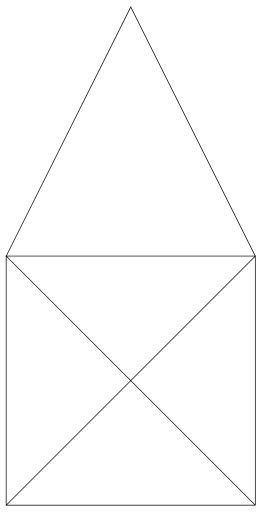
\includegraphics[width=2cm]{house/house.png}
	\caption{Das Haus}
	\label{fig:house}
\end{figure}
\label{sec:houses}
\end{document}